\chapter{MT-SOM semi-supervised model experiment}

\label{chap:mt-exp}

In this chapter, we focused on experiments with model MT-SOM which we briefly introduced in section \ref{our-approach}. In that section, we described the main components of the MT-SOM model, such as pre-trained SOM, feature vector input and SOM-based loss. In the following chapters \ref{chap:mlp-som} and \ref{chap:som-fv-cifar}, we discovered some of the concepts in simple setups and proved them. Based on these results, in this chapter, we specified details of the model and came up with experimental results.

\section{SOM loss for semi-supervised learning}
Since the SOM loss developed in chapter \ref{chap:mlp-som} was used only in supervised setup and computation of this loss needed to know classes of each data sample to create triplets, it was not possible to use it without modification in semi-supervised setup. That was because some of the training data had unknown classes - they were unlabeled. We proposed a new form of SOM-based loss, which is more suitable for a semi-supervised learning setup.

The input of loss was one input sample augmented in two different ways. Same as in the Binary mean teacher experiment \ref{chap:bmt-exp}, we used random rotation and random flip. For this pair of augmented images, we knew, that they belonged to the same class since they were only two modifications of the same image. Based on that, we wanted the distance of winner neurons on the SOM map to be minimal. 

Another information, that SOM loss reflected was how good is input represented by its winner neuron. That means, how good the prototype is and how relevant the winner distance information is. This information can be computed as the Euclidean distance of winner weights and input, since each SOM neuron`s weights have the same dimensionality as the inputs and represent a point in n-dimensional space. In SOM training, the neuron weights are adjusted in such a way, that they represent a group of inputs in this n-dimensional space better. So at the end of the training, the distance between the input and prototype means, how well the input is represented by the prototype.

We proposed SOM loss that combines these two pieces of information in equation \ref{som-loss-semi}. Two augmentations of the same input are denoted $x$ and $\xi$. Positions of winners on the map are denoted by the star symbol. The weights of neuron $i$ are denoted $w(i)$.

\begin{equation} \label{som-loss-semi}
\begin{split}
    J_{S2}(\tau) = || g(x, \tau)^* - g(\xi, \tau)^* ||^2 + \\[10pt]
    \psi \cdot || g(x, \tau) - w(g(x, \tau)^*) ||^2 +  \\[10pt]
    \psi \cdot || g(\xi, \tau) - w(g(\xi, \tau)^*) ||^2
\end{split}
\end{equation}


Supervised loss $S(\theta)$ is cross entropy loss already shown at equation \ref{eq:mt-loss-super}. Final loss is combined as shown in \ref{eq:mt-som-loss-sum}.

\begin{equation}
	Loss(\theta) = S(\theta) + \kappa(t) \cdot J_{S2}(\tau),
	\label{eq:mt-som-loss-sum}
\end{equation} 


\section{Experimental task}
In this section, we tested our model on a standard semi-supervised classification task with image dataset CIFAR-10 described in section \ref{dataset-cifar10}. We tested model performance on setup with $4\,000$, $1\,000$ labeled samples in the training set.


\section{Implementation and Model architecture}
Implementation of this model is an adaptation of Mean teacher code in Sarmads repository \cite{sarmad-repo}. 
We decided to use Sarmads implementation instead of Mean teacher authors' original implementation \cite{curiousai}, because the original model had over $30$ million parameters, which was very demanding on computational power. On the contrary, Sarmad's implementation used architecture with approximately $3$ million weights, and the code was tested and worked well in our experiment with the Binary mean teacher model. In chapter \ref{chap:bmt-exp}, there was Sarmad's model architecture described in detail in table \ref{layers}. 

We published adapted code in our repository \cite{dt-mt-repo}, in folder \\ \texttt{pytorch/experiments/semisup}. The experiment is divided into $4$ steps corresponding to Python scripts in the repository.
\begin{enumerate}
    \item Mean teacher model pre-training: To obtain feature vectors, we used the Mean teacher model, which is pre-trained for $10$ epochs with the labeled part of the training dataset. Pre-training is done by running script \texttt{supervised.py}.
    \item SOM from feature vectors training: Since we can produce feature vectors from the pre-trained MT model, we can train the SOM model. That is done by running script \texttt{som\_from\_fv.py}, which creates feature vectors and trains the SOM model for $100$ epochs.
    \item MT-SOM model training: With pre-trained SOM, we can train our semi-supervised model for $200$ epochs by running script \texttt{mt-som.py}.
\end{enumerate}


\section{Experimental results}

In this section, we focused on experimentation with the MT-SOM model and comparison of its results with a supervised baseline. Supervised baseline is an MT-like model that uses only supervised loss in the training of student networks. The teacher network is the exponential moving average of the student model. We investigate several values of $\kappa$ and $\psi$ hyperparameters, $2$ labeled portions and two types of $\kappa$ ramping. In these experiments, the shown results are results from $1$ trained model in setup with described hyperparameters, not the mean from more than one training. This is because the model is very rich in its parameters and training lasts approximately $4.5$ hours.


\begin{figure}[h!]
    \centering
    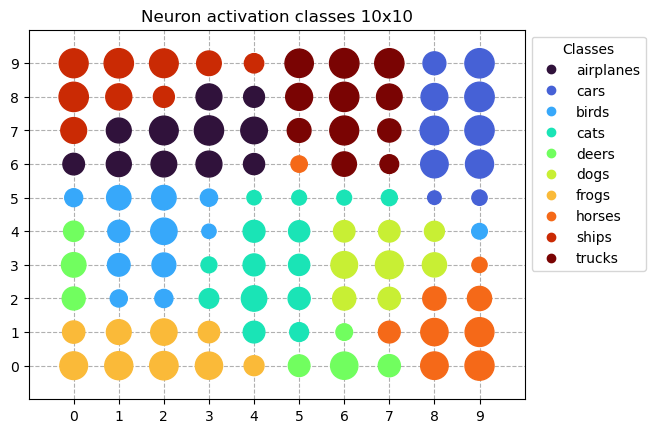
\includegraphics[width=0.8\linewidth]{figs/fv-10n-79ep-4000labeled.png}
    \caption{Experiment 1: Pre-trained Self-organizing map}
    \label{fig:exp1-som}
\end{figure}

\subsection{Experiment 1: Rampdown types of kappa}
\label{exp1}
In this first experiment, we compared the supervised baseline ($\kappa=0, \psi=0$) with the MT-SOM model which uses the first type of SOM-based loss. We used $4\,000$ labeled samples, which were specified in file \texttt{4000\_balanced\_labels/00.txt} Sarmads repository, which specify which images are used in the labeled part of the training set. We pre-trained the Mean teacher model on this data in a supervised setup. MT model achieved accuracy $66\%$. We took feature vectors from the model and trained a Self-organizing map. From the map shown in figure \ref{fig:exp1-som}, we can see, that SOM is well organized. In this experiment, we compared linear and sigmoid ramp down of $\kappa$. Hyper-parameter $\psi$ was not ramped. 

We run experiments with several $\kappa$ and $\psi$ hyperparameter values. Results of training with linear ramp-down are in table \ref{exp1-tab}. The table contains the best accuracies of the teacher model with specific $\kappa$ and $\psi$ values. We can see that supervised baseline accuracy is $81.14\%$ and the accuracy of the best model is $81.06\%$, which is approximately $0.9\%$ better. 


\begin{table}[h!]
\centering
\begin{tabular}{|c|c|c|c|c|c|}
\hline
$\kappa | \psi$ & 0       & 0.1     & 1       & 10      & 30      \\ \hline
0           & 81.14\% & ---     & ---     & ---     & ---     \\ \hline
0.1         & 81.38\% & 81.42\% & 81.22\% & 81.06\% & ---     \\ \hline
1           & 80.76\% & 81.32\% & 81.08\% & 81.98\% & ---     \\ \hline
5           & 81.36\% & 81.32\% & \color{purple}  82.00\% & \color{purple} 82.06\% & ---     \\ \hline
10          & ---     & ---     & 81.84\% & \color{purple}  82.00\% & 81.84\% \\ \hline
\end{tabular}
\caption{Linear ramp-down: Best accuracy of teacher model}
\label{exp1-tab}
\end{table}

Table \ref{exp1-tab-sigm} shows results of training with specific $\kappa$ and $\psi$ values and sigmoid ramp-down of $\kappa$. We can see that the baseline is the same as for linear ramp-down, but the best-performing model has an accuracy of $81.84$, which is only $0.7\%$ better than the baseline. Therefore, this experiment shows, that linear ramp-down of $\kappa$ provided better results of the semi-supervised model.


\begin{table}[h!]
\centering
\begin{tabular}{|c|c|c|c|c|c|}
\hline
$\kappa | \psi$ & 0       & 0.1     & 1       & 10      & 30      \\ \hline
0           & 81.14\% & ---     & ---     & ---     & ---     \\ \hline
5           &  --- & 81.72\% & 81.72\% &  81.60\% & ---     \\ \hline
10          & ---     & 81.28\% & \color{purple}81.84\% & 81.56\% & ---  \\ \hline
20         &  ---  & 81.30\% &  \color{purple}81.76\% & 81.68\% & ---     \\ \hline

\end{tabular}
\caption{Sigmoid ramp-down: Best accuracy of teacher model}
\label{exp1-tab-sigm}
\end{table}


In figure \ref{exp1-acc}, there were shown progress plots of both the student and the teacher model of baseline and the best-performing model ($\kappa=5, \psi=10$, linear ramp-down) during $200$ training epochs. We can see the comparison of the students' networks on the left side. MT-SOM model has very varying accuracy since the baseline is more stable. On the right side of the figure, there is a comparison of teacher networks. We can see that the exponential moving average in the MT-SOM model helps to stabilize varying student accuracies. Curves are quite similar, but the MT-SOM model provides better accuracy in most of the training epochs.


\begin{figure}[h!]
    \centering
    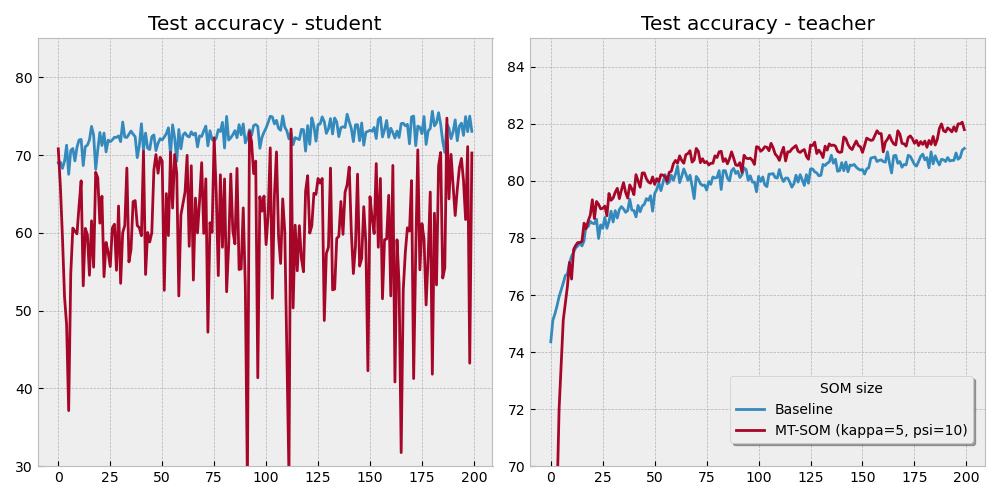
\includegraphics[width=0.8\linewidth]{figs/fv-som-acc.png}
    \caption{Experiment 1: Comparison of baseline and best model accuracy}
    \label{exp1-acc}
\end{figure}

In figure \ref{exp1-loss}, we can see progress plots of the loss function during the $200$ epoch of training. The leftmost plot shows the total loss value. The plot in the middle is supervised loss $S(\theta)$ and the plot on the right is the consistency SOM-based loss $J_{S2}(\tau)$ value progress. We can see, that both all the losses have a decreasing trend. Based on the curves, we can see, that total loss of the MT-SOM model is mostly influenced by SOM-based consistency loss and supervised loss only adds a minor value to the total value.

\begin{figure}[h!]
    \centering
    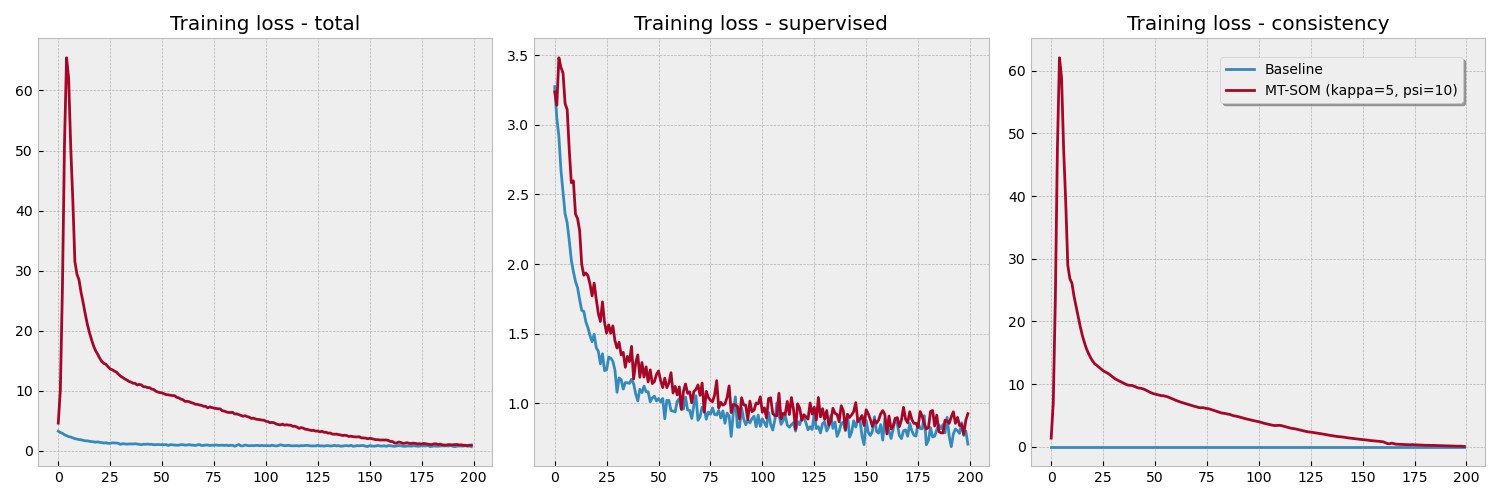
\includegraphics[width=1\linewidth]{figs/fv-som-loss.png}
    \caption{Experiment 1: Comparison of baseline and best model loss}
    \label{exp1-loss}
\end{figure}

\subsection{Experiment 2: 1000 labeled samples}

In this experiment, we focused on a smaller portion of labeled data. The training set contained only $1\,000$ labeled samples. Samples chosen as labeled were specified in file \texttt{1000\_balanced\_labels/00.txt}. Since the training set changed, it was not possible to use the same pre-trained Mean teacher model and Self-organizing map. Therefore we pre-trained the MT model on the new training set in the supervised setup. The accuracy of the model was $53\%$. Then we pre-trained SOM using feature vectors from pre-trained MT. Figure \ref{exp2-som} shows the map, which is quite well organized.

\begin{figure}[h!]
    \centering
    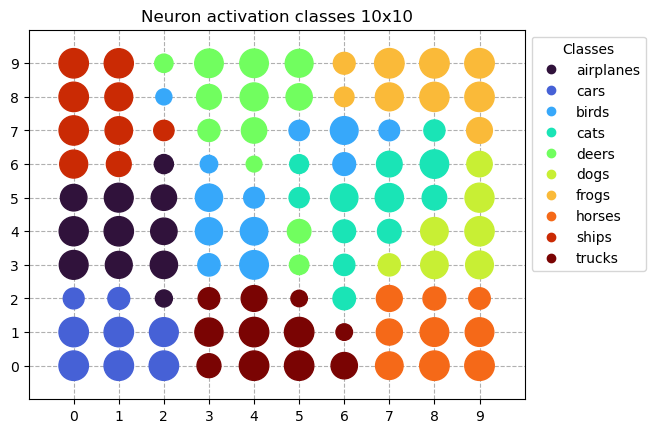
\includegraphics[width=0.8\linewidth]{figs/fv-10n-79ep.png}
    \caption{Experiment 2: Pre-trained Self-organizing map (1000 labeled samples)}
    \label{exp2-som}
\end{figure}

In this setup, we experimentally studied models with different values of hyperparameters. Table \ref{exp2-tab-lin} shows results of models with linear ramp-down of hyperparameter $\kappa$, whereas table \ref{exp2-tab-sigm} shows results of models with sigmoid ramp-down. The baseline best accuracy of the teacher model was $65.46\%$. 
The best performing MT-SOM model with linear ramp-down of $\kappa$ had accuracy $66.88\%$, which is more than $1.3\%$ better than the baseline. It was a model with hyperparameters  $\kappa=10$ and $\psi=5$. In the sigmoid ramp-down setup, the best performing MT-SOM model had hyperparameters $\kappa=1$ and $\psi=10$ with accuracy $66.48\%$, which is more than $1\%$ better than baseline.

\begin{table}[h]
\centering
\begin{tabular}{|c|c|c|c|c|}
\hline
$\kappa | \psi$ & 0    & 5       & 10      & 30      \\ \hline
0           & 65.46\%   & ---     & ---     & ---     \\ \hline
1           & ---   & 65.70\%     & 66.36\%     & 65.90\%     \\ \hline
10          & ---   & \color{purple} 66.88\% &  66.54\% & \color{purple} 66.60\%  \\ \hline

\end{tabular}
\caption{Linear ramp-down: Best accuracy of teacher model}
\label{exp2-tab-lin}
\end{table}


\begin{table}[h]
\centering
\begin{tabular}{|c|c|c|c|c|}
\hline
$\kappa | \psi$ & 0    & 5       & 10      & 30      \\ \hline
0           & 65.46\%   & ---     & ---     & ---     \\ \hline
1           & ---   & 65.94\%     & \color{purple} 66.48\%     & 65.52\%     \\ \hline
10          & ---   & 66.06\% & \color{purple} 66.36\% & 65.62\%  \\ \hline

\end{tabular}
\caption{Sigmoid ramp-down: Best accuracy of teacher model}
\label{exp2-tab-sigm}
\end{table}

We plotted the metrics of the best performing MT-SOM model ($\kappa=10, \psi=5$) and the baseline in the following figures \ref{exp2-acc} and \ref{exp2-loss}. In the first one, there was shown comparison of the accuracies of models during $200$ epochs of training. We can see similar behavior as in plots of previous experiment. The test accuracy of the student network of the MT-SOM model change is frequent. The teacher plots had more visible trends and the MT-SOM model was higher than the baseline during the whole training. The second figure \ref{exp2-loss} shows losses of compared models. We can see, that total loss had a decreasing trend in both models. We can also see, that supervised loss is very chaotic in both models.


\begin{figure}[h!]
    \centering
    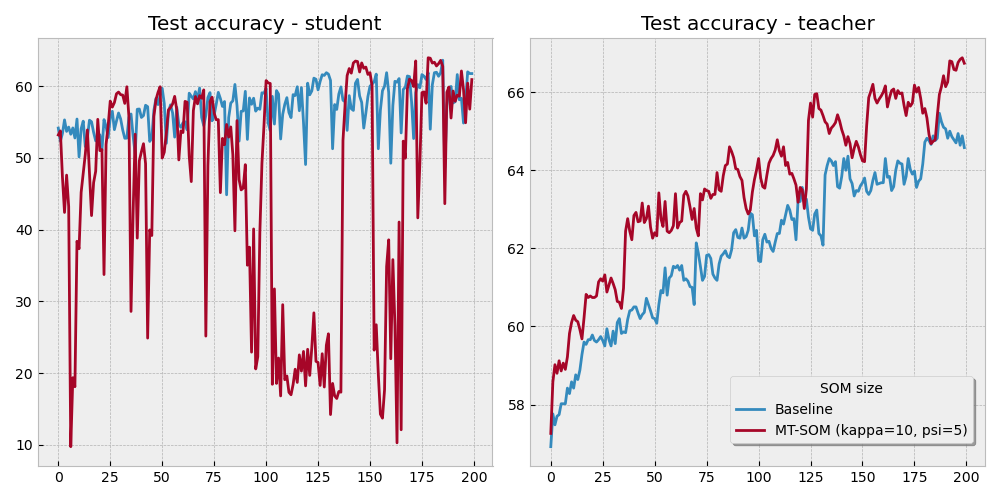
\includegraphics[width=0.8\linewidth]{figs/fv-som-acc-exp2.png}
    \caption{Experiment 2: Comparison of baseline and best model accuracy}
    \label{exp2-acc}
\end{figure}


\begin{figure}[h!]
    \centering
    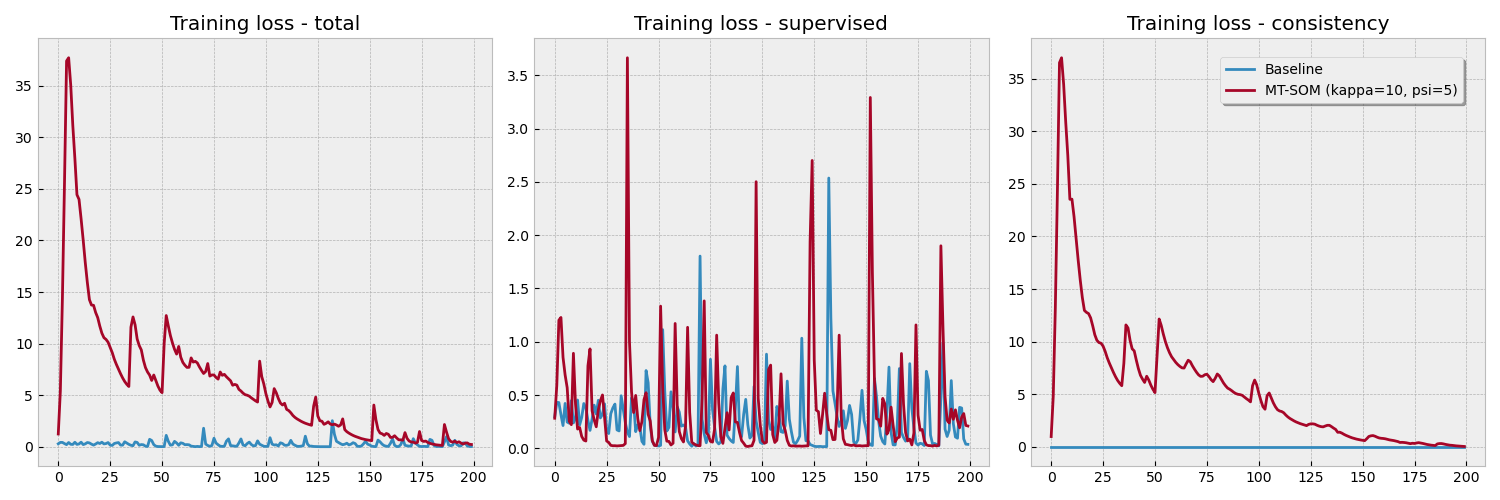
\includegraphics[width=1\linewidth]{figs/fv-som-loss-exp2.png}
    \caption{Experiment 2: Comparison of baseline and best model loss}
    \label{exp2-loss}
\end{figure}

\subsection{Experiment 3: Mean accuracy of setups}

In this experiment, we build on results from previous experiments 1 and 2. We decided to look further at MT-SOM models with promising hyperparameters, which are marked by purple color in result tables \ref{exp1-tab}, \ref{exp1-tab-sigm}, \ref{exp2-tab-lin} and \ref{exp2-tab-sigm}. We wanted to strengthen the credibility of these results which show the benefits of our MT-SOM model. We decided to rerun experiments, such that each hyperparameter setup had results of $3$ and we have shown the mean accuracy and the standard deviation of $3$ runs. We listed the results in table \ref{mean-results}. Each row represented one combination of hyperparameters. The first $4$ columns described the hyperparameters of the model. In cases when $\kappa=0$ and $\psi=0$, it was the baseline model. The results have shown, that the MT-SOM model overcame the baseline in both labeled portions. When it comes to $4\,000$ labels, the baseline was approximately $0.8\%$ worse than the best-performing MT-SOM model. In a setup with $1\,000$ labeled samples, the MT-SOM model has even better results compared to the baseline. The difference was more than $2\%$.


\begin{table}[]
\begin{tabular}{|c|c|c|c|c|c|c|c|}
\hline
Labeled & Rampdown & $\kappa$ & $\psi$   & 1. training & 2. training & 3. training & mean $\pm$ std \\ \hline
4\,000          & ---      & 0     & 0   &    81.14\%       &      81.12\%        &     81.24\%        & 81.17\% $\pm$ 0.05\%                \\ \hline
4\,000          & linear      & 5     & 1   &    82.00\%       &    81.68\%         &    81.72\%         &   81.80\% $\pm$ 0.14\%                 \\ \hline
4\,000          & linear      & 5     & 10   &   82.06\%        &     81.64\%        &    81.84\%         &   81.85\% $\pm$ 0.17\%                 \\ \hline
4\,000          & linear      & 10     & 10   &  82.00\%         &    81.98\%          &  81.80\%           &       81.93\% $\pm$ 0.09\%             \\ \hline
4\,000          & sigmoid      & 10     & 1   &  81.84\%         &    81.58\%          &      81.50\%       &   81.64\% $\pm$ 0.15\%                 \\ \hline
4\,000          & sigmoid      & 20     & 1   &  81.76\%         &     81.86\%        &    82.24\%         &    81.95\% $\pm$ 0.21\%                \\ \hline

1\,000          & ---      & 0     & 0   &    65.46\%       &    64.76\%         &     64.34\%         & 64.85\% $\pm$ 0.46\%                \\ \hline
1\,000          & linear   & 10    & 5   &    66.88\%        &       66.20\%       &   66.36\%            & 66.48\% $\pm$ 0.29\%           \\ \hline
1\,000          & linear   & 10    & 30  &    66.60\%         &       66.02\%        &       66.24\%        &       66.29\%  $\pm$ 0.43\%    \\ \hline
1\,000          & sigmoid  & 1     & 10  &    66.48\%         &      66.70\%       &      65.98\%        &   66.39\% $\pm$ 0.30\%         \\ \hline
1\,000          & sigmoid  & 10    & 10  &    66.36\%         &     67.04\%        &      67.54\%       &      66.98\% $\pm$ 0.48\%      \\ \hline

\end{tabular}
\caption{Experiment 3: Accuracies of models}
\label{mean-results}
\end{table}


%\subsection{Experiment 3: Loss type 2}

%In this experiment, we suggested trying another proposition of SOM-based loss, since we found it intuitively more suitable than the previous one. We denoted the error of the winner selection as $E_W$ and defined it in equation \ref{err-win}. New SOM-based loss is described in equation \ref{som-loss-semi2}. The idea behind the loss is that since both inputs $x$ and $\xi$ are augmentations of the same input, they belong to the same class. Therefore they should be close on the SOM map. But, since the feature vectors evolve in time, because of the model training, but the SOM stays the same, the winner selection error can increase. In that 


%\color{red} 

%VZDY SU VSTUPY Z ROVNAKEJ TRIEDY
%cim horsie su repr. prototypom, tym menej by nam informacia o prototypoch mala hovorit a nie ze tym vacsia je loss, teda aj chyba

%\color{black}

%\begin{equation}
%    E_W = || g(x, \tau) - w(g(x, \tau)^*) ||^2 + || g(\xi, \tau) - w(g(\xi, \tau)^*) ||^2
%    \label{err-win}
%\end{equation}


%\begin{equation}
%    J_{S3}(\tau) = \kappa(t) \cdot || g(x, \tau)^* - g(\xi, \tau)^* ||^2 \cdot (1 - \frac{1}{1+e^{-(E_W - B)}})
%    \label{som-loss-semi2}
%\end{equation}



%Max distance in SOM from exp 3 = (8.743154525756836, (0, 99))
%Min distance in SOM from exp 3 = (0.09822241961956024, (58, 59))

%Border hladame medzi 0.5 a 8.5 . 


%\begin{table}[h]
%\centering
%\begin{tabular}{|c|c|c|c|c|c|}
%\hline
%$\kappa | B$ & 0    & 1       & 2      & 3  & 5     \\ \hline
%0           & 65.46\%   & ---     & ---     & --- &     \\ \hline
%0.1           & ---   & 64.78\%     & 64.48\%     & 64.56\%  & 64.54\%  \\ \hline
%1           & ---   &  63.92\%     & 64.68\%     & 64.42\% &  64.72\%  \\ \hline
%10          & ---   & 64.48\% &64.24\% &64.58\% & 64.46\% \\ \hline

%\end{tabular}
%\caption{Best accuracy of teacher model}
%\end{table}

\section{Discussion}
From the results in this chapter, it can be inferred, that SOM-based loss helped the performance of the model in semi-supervised learning. We studied this concept of the MT-SOM model that uses self-organization to improve learning in several setups and proved it. The results have shown, that the combined model can scale the performance up by $0.5-2\%$, which can be a big improvement in cases when not enough data are available for supervised learning. We surely can say, that this model has the potential to be used in such situations and we believe that further study of the model is meaningful.